\documentclass[parskip=full]{scrartcl}
\usepackage[top=2.5cm, bottom=2.5cm, left=2.5cm, right=2.5cm]{geometry}
\usepackage[utf8]{inputenc}
\usepackage[T1]{fontenc}
\usepackage[german]{babel}
\usepackage[pangram]{blindtext}
\usepackage{hyperref}
\usepackage[toc, nonumberlist, numberedsection]{glossaries}
\usepackage{graphicx}
\usepackage{enumitem}

\hypersetup{
  colorlinks=false,
  linktoc=all,
  hidelinks,
}

%!TEX root = Pflichtenheft.tex

\newglossaryentry{Dockerimage}
{
  name=Dockerimage,
  plural=Dockerimages,
  description={Ein Container mit Programmen, der unabhängig vom zugrunde liegenden Betriebssystem gleichbleibende Bedingungen herstellt}
}

\newglossaryentry{Fertigungssimulation}
{
  name=Fertigungssimulation,
  plural=Fertigungssimulationen,
  description={Darstellung der Industrieanlage und Simulieren des Verhaltens}
}


\newglossaryentry{GUI}
{
  name=GUI,
  plural=GUIs,
  description={Die grafische Benutzerumgebung des Programms, welche vom Bediener gesehen wird}
}

\newglossaryentry{Industrial Data Space}
{
  name=Industrial Data Space,
  plural=Industrial Data Spaces,
  description={Eine Infrastruktur zum Austausch von Daten in der Industrie}
}

\newglossaryentry{Jitter}
{
  name=Jitter,
  description={Simulation von variierenden Werten, um näher an echten Anlagen zu liegen}
}

\newglossaryentry{Makro}
{
  name=Makro,
  plural=Makros,
  description={Eine aufgezeichnete Folge von Einstellungen, die gesetzt werden. Wird benutzt, um einen komplexeren Ablauf in der Anlage zu simulieren}
}

\newglossaryentry{OPC UA}
{
  name=OPC UA,
  plural=OPC UA,
  description={Ein Protokoll zur Übertragung von Daten und Steuersignalen von Industrieanlagen}
}

\newglossaryentry{Produktionsanlage}
{
  name=Produktionsanlage,
  plural=Produktionsanlagen,
  description={Großmaschinen, wie sie in der Industrie eingesetzt werden. Hier symbolisiert durch Tanks mit Flüssigkeiten}
}

\newglossaryentry{Sensordatum}
{
  name=Sensordatum,
  plural=Sensordaten,
  description={Ausgabewert eines simulierten Sensors wie Temperatur oder Durchflussmenge}
}

\newglossaryentry{Systemadapter}
{
  name=Systemadapter,
  plural=Systemadapter,
  description={Konvertiert die Daten eines Gesamtsystems (hier Industrieanlage) in ein anderes Format}
}

\newglossaryentry{TCP/IP Verbindung}
{
  name=TCP/IP Verbindung,
  plural=TCP/IP Verbindungen,
  description={Ein Protokoll zum Datenaustausch über das Internet}
}

\newglossaryentry{Uberwachungskonsole}
{
  name=Überwachungskonsole,
  plural=Überwachungskonsolen,
  description={Anzeige der Sensorwerte der Fertigungssimulation}
}

\newglossaryentry{Wrapper}
{
  name=Wrapper,
  plural=Wrapper,
  description={Programm, das ein anderes Programm umgibt und auf Ereignisse im umgebenen Programm reagieren kann}
}
\makeglossaries

\title{Pflichtenheft}
\subtitle{Implementierung eines OPC UA \glslink{Systemadapter}{Systemadapters} für den \gls{Industrial Data Space}}
\author{
    M. Armbruster\\
    D. Kahles\\
    H. Lehmann\\
    M. Schwarzmann\\
    N. Wilhelm
}

\begin{document}
\maketitle
\tableofcontents
\pagebreak

\section{Einleitung}
In der heutigen Zeit dringt die Vernetzung in immer neue Bereiche vor. So auch in die Industrie und ihre Fertigungsprozesse.
Dabei soll das Projekt Industrial Data Space helfen, einen Datenraum zu erzeugen, der Datensicherheit, Datensouveränität und
Transparenz bietet. Auf diese Weise soll dazu beigetragen werden, Industrie 4.0 voranzutreiben und somit durch Vernetzung von
Maschinen, Computern und Menschen die Leistungsfähigkeit der Industrie zu erhöhen und auf die Zukunft auszurichten.
Dabei hilft das auf TCP/IP basierende Kommunikationsprotokoll OPC UA, Maschinen miteinander interagieren zu lassen.

Die hier vorgestellte Simulation ermöglicht es, die Vorteile der Vernetzung von Maschinen mit OPC UA zu demonstrieren und zu verdeutlichen, um Industriekunden von den neuen Möglichkeiten zu überzeugen.
Die Hauptkomponenten sind ein Server (Fertigungssimulation) und ein Client (Überwachungskonsole),
die jeweils eine graphische Benutzeroberfläche (GUI) besitzen und auf getrennten Maschinen laufen können.
Sie kommunizieren lediglich über OPC UA.
In der GUI der Fertigungssimulation wird ein industrieller Prozess dargestellt.
Drei Tanks werden mit je einer farbigen Flüssigkeit gefüllt und leiten diese in einen weiteren Tank,
in dem die Flüssigkeiten durch einen Motor gemischt werden. Daten und Werte des Prozesses werden ebenfalls angezeigt. Dazu gibt es
die Möglichkeit, die Produktion zu konfigurieren,  zum Beispiel indem man Zu- und Abflussmengen oder Grenzen für Füllstände einstellt. Die visuelle Darstellung passt sich an die Konfiguration an.
Die Überwachungskonsole liest die Daten der Fertigungssimulation, stellt sie optisch ansprechend in einem Monitoring dar
und kann Alarme anzeigen, falls Grenzwerte überschritten werden. Das Monitoring ist ebenfalls konfigurierbar. Es ist etwa möglich, Filter auf Variablen anzuwenden. Allerdings hat die Überwachungskonsole keinen Einfluss auf die Fertigungssimulation.


\section{Zielbestimmung}
Der \gls{Systemadapter} dient dem Ziel, die Funktion von \gls{OPC UA} zu demonstrieren, ohne eine konkrete \gls{Produktionsanlage}
benutzen zu müssen. Somit kann beim Kunden das Protokoll flexibler vorgestellt werden. Hierzu soll das Programm
sowohl eine \gls{Produktionsanlage} simulieren und den Status grafisch darstellen, als auch auch eine Überwachungskonsole
bereitstellen, die über OPC UA Werte der Anlage abfragt.\\
\begin{center}
    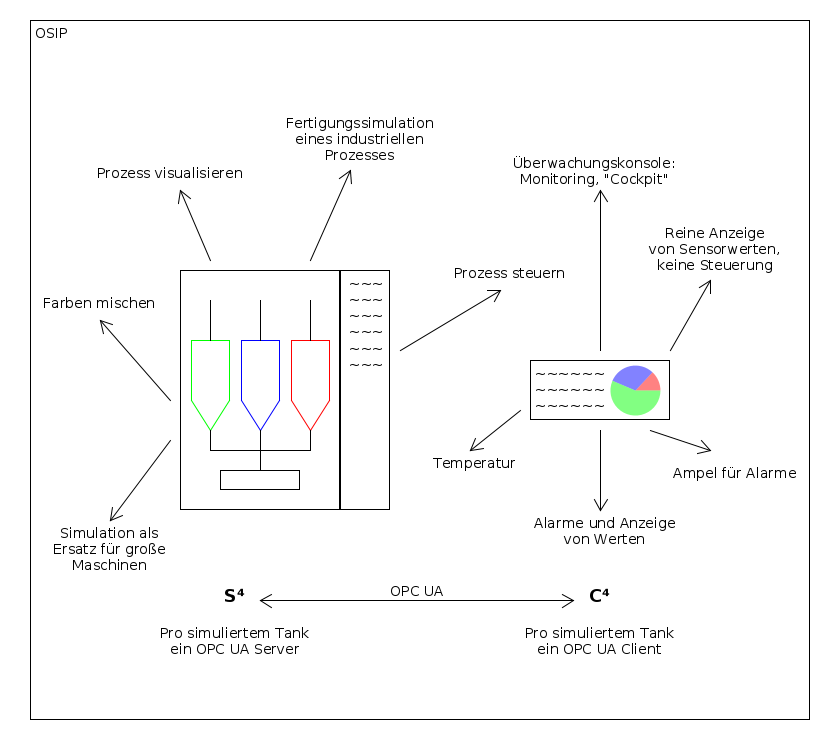
\includegraphics[scale=0.5]{../system-sketch.png}
\end{center}

\newpage
\section{Produkteinsatz}
\subsection{Anwendungsbereiche}
Das Produkt wird verwendet, um \gls{OPC UA} und dessen Möglichkeiten zu präsentieren.
Insbesondere soll es einfacher aufzubauen und zu zeigen sein als reale \glspl{Fertigungssimulation}.
Dies kann zum Beispiel auf Messen oder direkt bei potenziellen Kunden geschehen.
\subsection{Zielgruppen}
Die Zielgruppe umfasst Personen, die sich mit OPC UA auskennen und es potenziellen Anwendern vorführen möchten.
Dazu zählen insbesondere Mitglieder der OPC Foundation, die die Verbreitung des Protokolls fördern wollen,
aber auch Softwareentwickler die OPC UA konforme Software herstellen und möglichen Kunden auf einfache Art und
Weise die Funktionalität von OPC UA präsentieren wollen.
Die potenziellen Anwender haben meist keine Erfahrung mit OPC UA, sind aber für \glspl{Produktionsanlage} verantwortlich
die von OPC UA profitieren würden.

\subsection{Betriebsbedingungen}
Das Produkt kann entweder auf Messen, in Büros oder in Fertigungshallen direkt bei Kunden verwendet werden,
so lange die eingesetzte Hardware (siehe \ref{Hardware}) keine Probleme mit den Umgebungsbedingungen hat.

\section{Produktumgebung}
\subsection{Software}
Das Produkt erfordert einen Computer, auf dem das Betriebssystem Microsoft Windows 7, 8.1 oder 10 installiert ist,
oder auf dem Canonical Ubuntu 14.04 oder 16.04 installiert ist. Außerdem ist das Oracle Java Runtime Environment in Version 1.8
notwendig. Wenn die Fertigungssimulation und die Überwachungskonsole auf unterschiedlichen Computern laufen,
ist eine TCP/IP Verbindung mit einer Bandbreite von 100 MBit/s und einer Latenz von maximal 100 ms zwischen den Computern notwendig.
Außerdem wird eventuell (siehe \ref{fertigung-optional} und \ref{konsole-optional}) unter Ubuntu 16.04 die Containersoftware Docker
ab Version 1.10.3 unterstützt, mit dem die beiden Softwareteile isoliert in Containern verteilt und ausgeführt werden können.

\subsection{Hardware}
\label{Hardware}
Es ist ein Laptop oder Desktopcomputer notwendig, der eines der oben genannten Betriebssysteme unterstützt.
Zudem sind mindestens 2GB Arbeitsspeicher notwendig. Die CPU muss die x86 Architektur unterstützen, zwei Kerne haben und mit
mindestens 2GHz getaktet sein.

\section{Funktionale Anforderungen}
\subsection{Fertigungssimulation}
\subsubsection{Funktionalität}
\begin{enumerate}
\item[FA10] Die Zu- und Abflussmengen der oberen Flüssigkeitstanks können seperat eingestellt werden.
\item[FA20] Die Abflussmenge des unteren Flüssigkeitstanks kann eingestellt werden. Die Zuflussmenge ergibt sich aus der Summe der Abflussmengen der oberen Tanks.
\item[FA30] Der untere Tank enthält einen motorbetriebenen Mischer, dessen Drehzahl eingestellt werden kann.
\item[FA40] Jedem der oberen Tanks ist eine Flüssigkeitsfarbe zugeordnet. Die Farbe des unteren Tanks ergibt sich aus dem Mischungsverhältnis der oberen Tanks. Dabei wird
  angenommen, dass die Flüssigkeiten der oberen Tanks die selbe Deckkraft haben.
\item[FA50] Es gibt eine .jar Datei, die bei Ausführung die Fertigungssimulation startet.
\item[FA60] Nach Anforderung durch die \"Uberwachungskonsole wird in bestimmten, in der Anfrage definierten, Zust\"anden ein Alarm an die \"Uberwachungskonsole gesendet.
\item[FA70] Kommt es in der Simulation zu einem \"Uberlauf so h\"alt die Simulation an und es wird der Text ``\"Uberlauf'' angezeigt.
\item[FA80] Das System kann aus einem ``\"Uberlauf'' durch zur\"ucksetzen wieder in den Startzustand versetzt werden. Anschlie{\ss}end wird die Ausführung fortgesetzt.
\item[FA90] Eine \"Uberwachungskonsole kann sich bei der Fertigungssimulation registrieren, um von dieser Daten zu erhalten.
\item[FA100] Die Zuflusstemperaturen der oberen Tanks können seperat eingestellt werden.
\item[FA110] Die Füllstände der Tanks werden gemessen.
\item[FA120] Die Fertigungssimulation kommuniziert über OPC UA in einem TCP/IP Netzwerk mit Überwachungskonsolen.
\item[FA130] Der Port, \"uber den die Fertigungssimulation kommuniziert, kann eingestellt werden.
\end{enumerate}

\subsubsection{GUI Darstellung}
\begin{enumerate}
\item[FA110] Die GUI der Fertigungssimulation zeigt drei Tanks, die auf einer Höhe sind, und einen Tank unter den oberen drei.
Es führen Leitungen von den drei oberen Tanks zum unteren Tank.
\item[FA120] Der Mischer im unteren Flüssigkeitstank wird durch ein sich drehendes GUI Element dargestellt.
Die Umdrehungsgeschwindigkeit repräsentiert die Drehzahl des Mischermotors.
\item[FA130] Der Füllstand der Flüssigkeitstanks wird durch das Füllen der Tanks in der Farbe ihrer Flüssigkeit dargestellt.
\item[FA140] Die einstellbaren Parameter können in einem Unterfenster eingestellt werden. Darin existiert für jeden Tank ein eigener Reiter, der die 
tankspezifischen Einstellungen wie zum Beispiel Zu- und Abflussmengen, Zuflusstemperaturen oder Motordrehzahlen (siehe FA10 bis FA30) enthält.
Diese Parameter werden durch Schieberegler eingestellt.
\item[FA150] Jeder der dargestellten Tanks ist mit einer hellgrauen Box hinterlegt, welche den Zuständigkeitsbereich des jeweiligen OPC UA Servers repräsentiert.
\item[FA160] Die Fertigungssimulation besitzt einen ``Über''-Dialog, welcher Lizenzinfos zu verwendeten Bibliotheken,
  sowie eine kurze Information zu den Erstellern des Programms enthält.
\item[FA170] Die Fertigungssimulation besitzt einen Einstellungsdialog, der im Menü über ``Datei $\rightarrow$ Einstellungen'' angezeigt werden kann.
\item[FA180] Der Einstellungsdialog besitzt Buttons zum Verwerfen (``Abbrechen'') und Anwenden der Änderungen.
\item[FA190] Der Einstellungsdialog besitzt einen ``OK''-Button, welcher die Änderungen anwendet und den Dialog schließt.
\item[FA200] Der Einstellungsdialog besitzt einen Regler, welcher den \gls{Jitter} durch einen Schieberegler konfigurierbar macht.
  Hierbei entspricht ein \gls{Jitter} von 0 der Deaktivierung der Funktion.
\item[FA210] Der Einstellungsdialog besitzt eine Liste mit \glspl{Makro}. Daneben befinden sich Buttons zum Erstellen, Umbenennen und Löschen von \glspl{Makro}.
\end{enumerate}

\subsubsection{Optionale Funktionalität}
\label{fertigung-optional}
\begin{enumerate}
\item[FA240] Es gibt ein \gls{Dockerimage} zur einfachen Verteilung und isolierten Ausführung der Fertigungssimulation.
\end{enumerate}

\subsection{Überwachungskonsole}
\subsubsection{Funktionalität}
\begin{enumerate}
\item[FA310] Die \gls{Uberwachungskonsole} zeigt die Farbe der Flüssigkeitstanks an.
\item[FA320] Die \gls{Uberwachungskonsole} zeigt die Zu-, und Abflussmenge der oberen Flüssigkeitstanks an.
\item[FA330] Die \gls{Uberwachungskonsole} zeigt die Abflussmenge des unteren Flüssigkeitstanks an.
\item[FA340] Die \gls{Uberwachungskonsole} zeigt die Drehzahl des Mischermotors an.
\item[FA350] Alle angezeigten \glspl{Sensordatum} werden mit der eingestellten Aktualisierungsfrequenz aktualisiert.
\item[FA360] Der Benutzer kann die Anzeige der Füllstands- und Temperaturverläufe für jeden Tank ein- und ausschalten.
\item[FA370] Es gibt eine .jar Datei, die bei Ausführung die \gls{Uberwachungskonsole} startet.
\item[FA380] Es k\"onnen Alarme mit ihrem jeweiligen Ausl\"oser bei der Fertigungssimulation registriert werden.
\item[FA385] Bereits registrierte Alarme k\"onnen wieder gel\"oscht werden.
\item[FA390] Die \"Uberwachungskonsole kann sich unter Angabe einer IP-Adresse bei einer Fertigungssimulation im Netzwerk
  registrieren, um von dieser Daten zu erhalten.
\item[FA400] Die Überwachungskonsole kommuniziert über OPC UA in einem TCP/IP Netzwerk mit einer Fertigungssimulation. 
\item[FA410] Die Überwachungskonsole verbindet sich mit der Fertigungssimulation über deren IP Adresse. 
\item[FA420] Der Port der Überwachungskonsole kann eingestellt werden.
\end{enumerate}
\subsubsection{GUI Darstellung}
\begin{enumerate}
\item[FA410] Die \gls{Uberwachungskonsole} enthält für die Einstellungen ein getrenntes Fenster.
\item[FA420] Das Einstellungsfenster hat zwei Reiter: ``Allgemeines'' und ``Empfangene Daten''.
\item[FA430] Im Reiter ``Allgemeines'' kann die Aktualisierungsfrequenz eingestellt werden.
\item[FA440] Im Reiter ``Empfangene Daten'' kann für jeden Tank die Anzeige des Füllstands und des Temperaturverlaufs mittels Checkboxen ein- und ausgeschaltet werden.
\item[FA450] Im Reiter ``Alarme'' werden die aktuell registrierten Alarme aufgelistet.
\item[FA460] Im Reiter ``Alarme'' wird durch einen Klick auf das Feld ``Alarm registrieren'' der Dialog zur Erstellung eines
  neuen Alarms ge\"offnet.
\item[FA470] Im Reiter ``Alarme'' wird durch einen Klick auf den ``L\"oschen''-Button neben einem Alarm ein registrierter Alarm entfernt.
\item[FA480] Alarme werden synchron zu den Aktualisierungen der Werte empfangen.
\item[FA490] Empfangene Alarme werden im Logging-Fenster f\"ur Alarme angezeigt.
\end{enumerate}

\subsubsection{Optionale Funktionalität}
\label{konsole-optional}
\begin{enumerate}
\item[FA540] Es gibt ein \gls{Dockerimage} zur einfachen Verteilung und isolierten Ausführung der Überwachungskonsole
\end{enumerate}

\section{Nichtfunktionale Anforderungen}
\subsection{Fertigungssimulation}
\begin{enumerate}
 \item[NF10] Die Drehzahl des Mischermotors kann in einem Bereich zwischen 0 und 300 Umdrehungen pro Minute gewählt werden.
 \item[NF20] Wenn Parameter verändert werden, sind sie nach spätestens einer halben Sekunde per OPC UA abrufbar.
 \item[NF30] Wenn der Zufluss eines Tanks komplett geschlossen, und der Ablauf komplett geöffnet wird, ist der Tank in etwa 10 Sekunden leergelaufen.
 \item[NF40] Wenn der Zufluss eines Tanks komplett geöffnet, und der Ablauf komplett geschlossen wird, ist der Tank in etwa 10 Sekunden übergelaufen.
\end{enumerate}

\subsection{Überwachungskonsole}
\begin{enumerate}
 \item[NF110] Die Aktualisierungsfrequenz kann im Bereich zwischen 20 und 4000 Millisekunden gewählt werden.
 \item[NF120] Wenn sich Werte in der Fertigungssimulation ändern, werden die Änderungen spätestens nach der Zeitspanne von
   einer halben Sekunde plus dem Aktualisierungsintervall in der Überwachungskonsole angezeigt.
\end{enumerate}

\section{Produktdaten}
\begin{enumerate}
 \item[D10] Die Überwachungskonsole speichert die zuletzt eingestellte IP Adresse und den Port des Servers.
 \item[D20] Die Überwachungskonsole speichert die zuletzt angezeigten \glspl{Sensordatum}.
 \item[D30] Die Überwachungskonsole speichert die zuletzt aktivierten Alarme.
 \item[D110] Die Fertigungssimulation speichert den zuletzt genutzten Port.
 \item[D120] Die Fertigungssimulation speichert den zuletzt eingestellten \gls{Jitter}.
 \item[D130] Die Fertigungssimulation speichert \emph{eventuell (sofern implementiert)} aufgenommene \glspl{Makro}.
\end{enumerate}

\section{Globale Testfälle}
\Blindtext[1]

\section{Systemmodelle}
\subsection{Szenarien}
\subsubsection{Szenario 1: Unabhängige Installation}
Manuel möchte Philipp, einem Kunden aus der Industrie, zeigen, was mit modernen Industrie 4.0 Techniken möglich ist.
Da Philipp nur wenig Zeit hat, fährt Manuel mit dem Auto zu Philipp. Weil Manuel weder Platz 
noch Zeit für eine komplette Demonstrationsanlage hat, nimmt er einen Laptop mit Simulationssoftware mit.

Vor Ort angekommen, startet er auf dem Laptop zwei virtuelle Maschinen, auf denen je ein Programm installiert ist. 
Einmal eine Fertigungssimulation und auf der anderen virtuellen Maschine eine Überwachungskonsole, um die Fertigung zu überwachen.
Nun weist Manuel den beiden virtuellen Maschinen je eine feste IP-Adresse zu.
Anschlie{\ss}end startet Manuel erst die Fertigungssimulation und dann die Überwachungskonsole.
Beim Start der Überwachungskonsole wird er nach der IP-Adresse gefragt, unter der die Fertigungssimulation zu finden ist. 
Er gibt die Adresse der anderen virtuellen Maschine an und auch die Überwachungskonsole startet erfolgreich. 
Nun ist klar, dass die beiden Programme tatsächlich über das Netzwerk kommunizieren.

In der Fertigungssimulation wird nun eine Produktionsanlage angezeigt, in der Flüssigkeiten aus drei Tanks
in einem weiteren Tank vermischt werden; Farben des Inhalts der Ursprungs- und des Zieltanks visualisieren den Vorgang. 
Im Zieltank dreht sich ein Motor, der für die Durchmischung sorgt.
Es gibt Sensoren für Temperatur, Farbe, Füllstand und Durchfluss der Tanks sowie für die Drehzahl des Motors.
In der Überwachungskonsole sieht man nun eine Reihe von Feldern mit sich aktualisierenden Daten,
die Zu- und Abfluss, Farbe und Temperatur der verschiedenen Tanks zeigen.

\subsubsection{Szenario 2: Konfigurierbarkeit}
Als Philipp zu ihm kommt, will Manuel ihm die Funktion von OPC UA demonstrieren.
Als erstes ändert er in der Fertigungssimulation den Zu- und Abfluss bei zwei der Tanks. Nun sehen die beiden, wie
sich die von der Überwachungskonsole angezeigten Werte für Zu- und Abfluss mit der nächsten Aktualisierung ändern. Die
Farbe im Zielcontainer ändert sich langsam, während sich das Mischungsverhältnis der Flüssigkeiten ändert. Auch diese
Werte werden in der Überwachungskonsole jeweils aktualisiert.

Als nächstes navigiert Manuel in das Einstellungsmenü seines Clients. Dort geht er in den Punkt ``Empfangene Daten'' und
wählt zusätzlich zu den bisher angezeigten Werten noch die Kategorien ``Füllstand'' und ``Motordrehzahl'' beim unteren Tank
an. Nach einem Klick auf ``Übernehmen'' sehen die beiden, wie in der Überwachungskonsole neue Anzeigen aufgetaucht sind,
die die neuen Werte darstellen. Außerdem entsteht ein neuer Reiter bei der Überwachungsanzeige des unteren Tanks,
in dem Philipp den Füllstandsverlauf ansehen kann.

Philipp merkt nun an, dass ihm die Flexibilität der empfangenen Daten sehr gefällt. Das Aktualisierungsintervall von
einer Sekunde sei aber in manchen der Fertigungsprozesse zu lang, da in manchen kritischen Zuständen sehr schnell
automatisch reagiert werden muss, etwa wenn Schwellenwerte überschritten werden. Daraufhin ändert Manuel in den
Einstellungen das Aktualisierungsintervall von 1000ms auf 250ms. Anschließend sehen beide, wie sich die Werte in der
Überwachungskonsole tatsächlich vier Mal pro Sekunde aktualisieren.

\subsubsection{Szenario 3: Alarme}
Philipp ist zunehmend an OPC UA interessiert, hat aber noch letzte Zweifel. Er merkt an, dass die Abfrage der Daten
zwar gut funktioniert, eine wirkliche \"Uberwachung aber noch einen Wrapper f\"ur das Programm ben\"otigen w\"urde,
um ungew\"ohnliche Zust\"ande in der Fertigung automatisch zu bemerken und darauf aufmerksam zu machen.
Manuel merkt an, dass das ein guter Einwand ist und dass OPC UA auch daf\"ur eine passende Funktionalit\"at besitzt.

Er \"offnet das Einstellungsmen\"u der \"Uberwachungskonsole und erstellt einen neuen Alarm. Um die Flexibilit\"at
von OPC UA erneut zu demonstrieren fragt er Philipp, welchen Zustand er gerne abfangen w\"urde. Philipp w\"urde gerne
abfangen, wenn ein Tank \"uberzulaufen droht. Er schl\"agt daf\"ur als Grenze einen F\"ullstand von 95\% vor.
Manuel gibt also in der \"Uberwachungskonsole 95\% als Grenze an und w\"ahlt einen Tank, f\"ur den der Alarm stattfinden soll.
Dann speichert er die neuen Einstellungen.

Anschlie{\ss}end dreht er in der Fertigungssimulation den Zufluss des entsprechenden Tanks auf, woraufhin der F\"ullstand
zu steigen beginnt. In der Fertigungssimulation ist der steigende F\"ullstand zu sehen, in der \"Uberwachungskonsole werden
steigende Werte angezeigt.
Darauf wird der F\"ullstand von 95\% erreicht und in der \"Uberwachungskonsole der Alarm ausgel\"ost. Manuel
beschlie{\ss}t, nicht zu handeln und der Tank l\"auft \"uber. Danach w\"ahlt Philipp in den Einstellungen der
Fertigungssimulation die Option ``zur\"ucksetzen'' woraufhin wieder die Standardkonfiguration angezeigt wird.

\subsection{Anwendungsfälle}
\subsubsection{Änderung der Zu-/Abflussgeschwindigkeit}
\begin{description}
 \item[Name] Erhöhen oder Verringern der Zu- oder Abflussgeschwindigkeit bei einem der Flüssigkeitstanks.
 \item[Akteure] Manuel (Bediener der Software)
 \item[Eingangsbedingung] Die Fertigungssimulation und die Überwachungskonsole sind in Betrieb und miteinander verbunden.
 \item[Ereignisfluss]
 \begin{itemize}[noitemsep]
  \item Manuel öffnet in der Fertigungssimulation den Reiter ``Ansicht''.
  \item Manuel klickt auf ``Steuerung anzeigen''.
  \item Ein Fenster öffnet sich. Manuel wählt den Reiter des Tanks, den er verändern will.
  \item Manuel verschiebt den Schieberegler des Zufluss- oder Abflussventils auf den gewünschten Wert.
  \item Manuel klickt den ``OK'' Knopf.
 \end{itemize}
 \item[Ausgangssituation] Die Zu- oder Abflussrate im gewählten Tank ist nun höher bzw. niedriger. Dies ist am schnelleren oder langsameren Füllen oder Leeren des Tanks in der Visualisierung der Tanks sichtbar.
 Außerdem zeigt die Überwachungskonsole höhere/niedrigere Durchflussraten an.
 \item [Nichtfunktionale Anforderungen] Der geänderte Zu- oder Abflusswert wird mit der nächsten Aktualisierung auf der Überwachungskonsole angezeigt.
\end{description}

\subsubsection{Änderung der angezeigten Sensorwerte}
\begin{description}
 \item[Name] Hinzuwählen oder Abwählen von \glspl{Sensordatum}, die in der \gls{GUI} angezeigt werden.
 \item[Akteure] Manuel (Bediener der Software)
 \item[Eingangsbedingung] Die Fertigungssimulation und die Überwachungskonsole sind in Betrieb und miteinander verbunden.
 \item[Ereignisfluss]
 \begin{itemize}[noitemsep]
  \item Manuel öffnet in der Überwachungskonsole die Einstellungen.
  \item Ein neues Fenster erscheint. Manuel navigiert in den Reiter ``Empfangene Daten''.
  \item Manuel klickt auf die Haken in der Liste, um Sensorwerte hinzuzufügen oder auszublenden.
  \item Manuel klickt den ``OK'' Knopf.
 \end{itemize}
 \item[Ausgangssituation] Die \glspl{Sensordatum}, deren Haken entfernt wurden, werden sofort ausgeblendet. Die \glspl{Sensordatum}, deren Haken hinzugefügt wurden, erscheinen sofort in der \gls{GUI}.
 \item [Nichtfunktionale Anforderungen] Die geänderten Einstellungen werden binnen einer halben Sekunde in der \gls{GUI} dargestellt.
\end{description}

\subsubsection{Änderung der Aktualisierungsfrequenz}
\begin{description}
 \item[Name] Erhöhen oder Verringern der Aktualisierungsfrequenz.
 \item[Akteure] Manuel (Bediener der Software)
 \item[Eingangsbedingung] Die Fertigungssimulation und die Überwachungskonsole sind in Betrieb und miteinander verbunden.
 \item[Ereignisfluss]
 \begin{itemize}[noitemsep]
  \item Manuel öffnet in der Überwachungskonsole die Einstellungen.
  \item Manuel navigiert in den Reiter ``Allgemeine Einstellungen''.
  \item Manuel verschiebt den Schieberegler, der die Aktualisierungsfrequenz einstellt.
  \item Manuel klickt den ``OK'' Knopf.
 \end{itemize}
 \item[Ausgangssituation] Die Sensorwerte in der Überwachungskonsole werden nun in Abständen der gewählten Aktualisierungsfrequenz aktualisiert.
 \item [Nichtfunktionale Anforderungen] Die Frequenz ändert sich spätestens mit der nächsten Aktualisierung.
\end{description}

\subsubsection{Erstes Starten der Simulation auf virtuellen Maschinen}
\begin{description}
 \item[Name] Einrichtung und Starten der Simulation auf virtuellen Maschinen
 \item[Akteure] Manuel (Bediener der Software)
 \item[Eingangsbedingung] Eine virtuelle Maschine, auf der die JAR der Überwachungskonsole gespeichert ist und eine virtuelle Maschine, auf der die JAR der Fertigungssimulation gespeichert ist, sind in Betrieb und haben feste IP Adressen zugewiesen bekommen.
 \item[Ereignisfluss]
 \begin{itemize}[noitemsep]
  \item Manuel startet die JAR der Fertigungssimulation.
  \item Manuel startet die JAR der Überwachungskonsole.
  \item Manuel gibt die IP Adresse ein, unter der die Fertigungssimulation zu finden ist.
 \end{itemize}
 \item[Ausgangssituation] Die Fertigungssimulation und die Überwachungskonsole sind verbunden und laufen mit ihren Initialwerten.
 \item[Nichtfunktionale Anforderungen] Die Sensorwerte der Überwachungskonsole werden nach spätestens einer halben Sekunde aktualisiert.
\end{description}
 
\subsubsection{Alarm erstellen}
\begin{description}
 \item[Name] Erstellen eines neuen Alarms in der \gls{Uberwachungskonsole}.
 \item[Akteure] Manuel (Bediener der Software)
 \item[Eingangsbedingung] Die \gls{Fertigungssimulation} und die \gls{Uberwachungskonsole} sind in Betrieb und miteinander verbunden.
 \item[Ereignisfluss]
 \begin{itemize}[noitemsep]
  \item Manuel \"offnet in der \gls{Uberwachungskonsole} die Einstellungen.
  \item Manuel navigiert in den Reiter ``Alarme''.
  \item Manuel klickt den Knopf ``Neuen Alarm erstellen''.
  \item Manuel w\"ahlt den \gls{OPC UA} Server, zu dem der Alarm geh\"ort.
  \item Manuel w\"ahlt den Sensor, zu dem der Alarm geh\"ort.
  \item Manuel erstellt eine Regel zum Ausl\"osen des Alarms.
  \item Manuel klickt den ``\"Ubernehmen'' Knopf.
 \end{itemize}
 \item[Ausgangssituation] Wenn der Sensor die Alarmbedingung erf\"ullt, wird an die \gls{Uberwachungskonsole} ein Alarm gesendet.
 \item [Nichtfunktionale Anforderungen] Sp\"atestens nach 100ms ist die Aktualisierung \"ubernommen und wird
  an die \gls{Fertigungssimulation} gesendet.
\end{description}

\subsubsection{Alarm empfangen}
\begin{description}
 \item[Name] Empfangen eines Alarms in der \gls{Uberwachungskonsole}.
 \item[Akteure] \gls{Fertigungssimulation}
 \item[Eingangsbedingung] Die \gls{Fertigungssimulation} und die \gls{Uberwachungskonsole} sind in Betrieb und miteinander verbunden.
  Es ist mindestens ein Alarm eingerichtet.
 \item[Ereignisfluss]
 \begin{itemize}[noitemsep]
  \item In der \gls{Fertigungssimulation} kommt es zu einem Alarmzustand.
  \item Die \gls{Fertigungssimulation} sendet den entsprechenden Alarm an die registrierte \gls{Uberwachungskonsole}.
  \item Die \gls{Uberwachungskonsole} empf\"angt den Alarm.
  \item Die \gls{Uberwachungskonsole} zeigt in der \gls{GUI} den Alarm an.
 \end{itemize}
 \item[Ausgangssituation] \gls{Fertigungssimulation} und \gls{Uberwachungskonsole} laufen normal weiter. In der \gls{GUI} der
  \gls{Uberwachungskonsole} ist der Alarmeintrag zu sehen.
 \item [Nichtfunktionale Anforderungen] Die \gls{GUI} der \gls{Uberwachungskonsole} muss einen empfangenen Alarm nach sp\"atestens
  100ms anzeigen.
\end{description}

\subsubsection{Alarm \"andern}
\begin{description}
 \item[Name] \"Andern eines bereits vorhandenen Alarms in der \gls{Uberwachungskonsole}.
 \item[Akteure] Manuel (Bediener der Software)
 \item[Eingangsbedingung] Die \gls{Uberwachungskonsole} ist in Betrieb. Es ist mindestens ein Alarm bereits vorhanden.
 \item[Ereignisfluss]
 \begin{itemize}[noitemsep]
  \item Manuel \"offnet in der \gls{Uberwachungskonsole} die Einstellungen.
  \item Manuel navigiert in den Reiter ``Alarme''.
  \item Manuel klickt auf ``Alarme anzeigen''.
  \item Manuel w\"ahlt den gew\"unschten Alarm an.
  \item Der Button ``Alarm bearbeiten'' wird klickbar.
  \item Manuel klickt auf ``Alarm bearbeiten''.
  \item Manuel tr\"agt die gew\"unschten \"Anderungen ein.
  \item Manuel klickt auf \"Ubernehmen.
 \end{itemize}
 \item[Ausgangssituation] Die alte Alarmbedingung l\"ost keine Alarme mehr aus. Die neue Alarmbedingung l\"ost Alarme aus.
 \item [Nichtfunktionale Anforderungen] Die ge\"anderte Alarmbedingung ist nach sp\"atestens 100ms \"ubernommen undan
  wird an die Fertigungssimulation gesendet.
\end{description}

\subsubsection{Alarm l\"oschen}
\begin{description}
 \item[Name] L\"oschen eines bereits erstellten Alarms.
 \item[Akteure] Manuel (Bediener der Software)
 \item[Eingangsbedingung] Die \"Uberwachungskonsole ist in Betrieb. Es ist mindestens ein Alarm bereits vorhanden.
 \item[Ereignisfluss]
 \begin{itemize}[noitemsep]
  \item Manuel \"offnet in der \"Uberwachungskonsole die Einstellungen.
  \item Manuel navigiert in den Reiter ``Alarme''.
  \item Manuel klickt auf ``Alarme anzeigen''.
  \item Manuel w\"ahlt alle gew\"unschten Alarme.
  \item Manuel klickt auf ``Alarme l\"oschen''.
  \item Manuel klickt im folgenden Dialog auf ``Best\"atigen''.
 \end{itemize}
 \item[Ausgangssituation] Die alten Alarmbedingungen l\"osen keine Alarme mehr aus.
 \item [Nichtfunktionale Anforderungen] Die L\"oschung der Alarme wird nach sp\"atestens 100ms an die Fertigungssimulation \"ubermittelt.
\end{description}

\subsubsection{Anwendungsfalldiagramm}
\begin{center}
  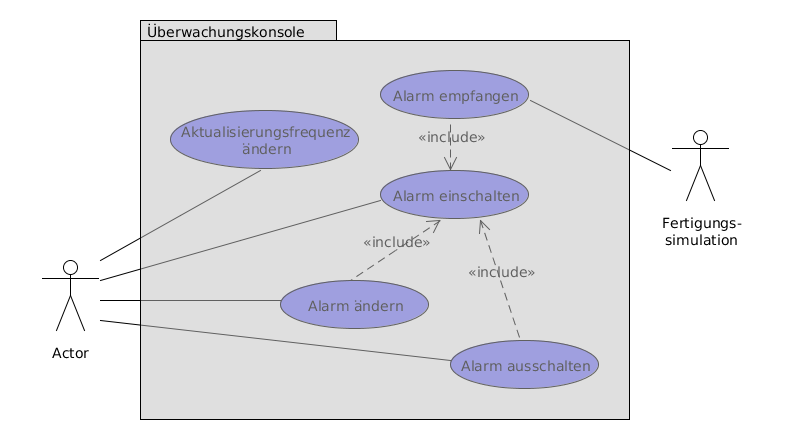
\includegraphics[scale=0.7]{media/UseCases/Ueberwachungskonsole.png}
\end{center}

\subsection{Dynamische Modelle}
\Blindtext[1]

\subsection{Statische Modelle}
\Blindtext[1]

\section{Nutzerinterface-Skizzen}
\subsection{Fertigungssimulation}
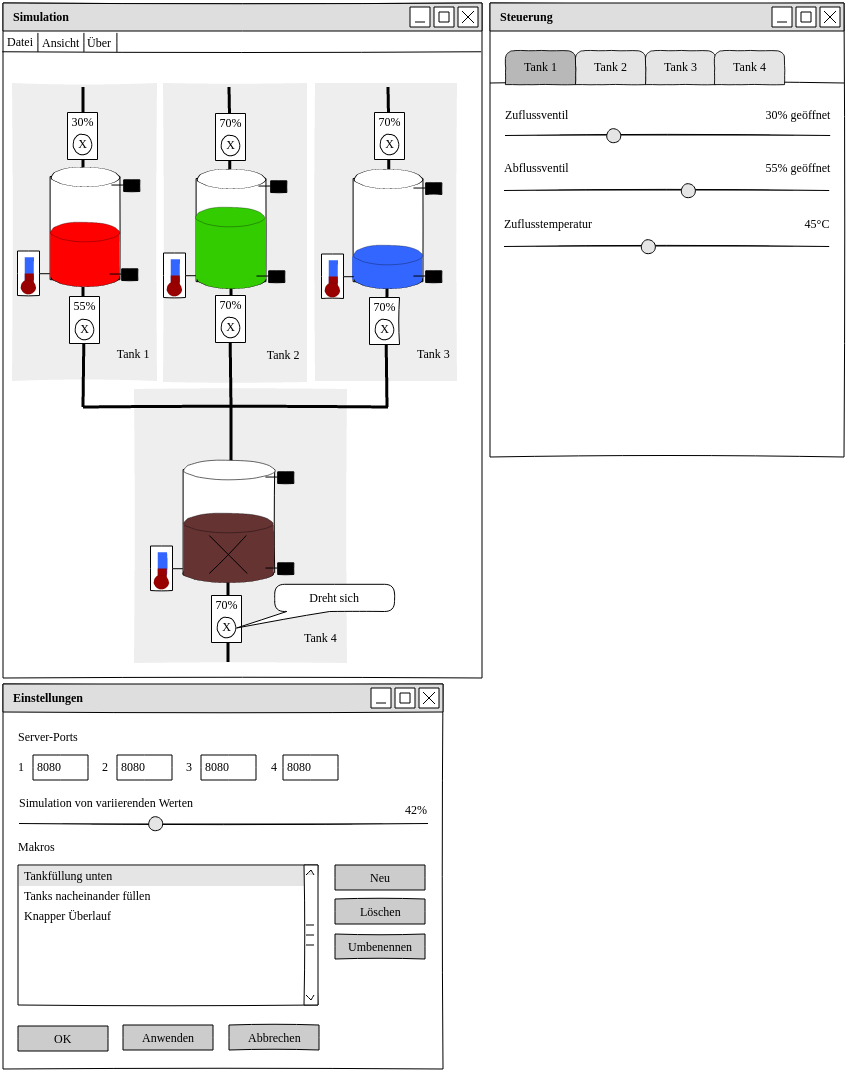
\includegraphics[scale=0.5]{media/ui-sketch-server.png}

\pagebreak
\printglossaries

\end{document}
